\subsection{Kenngrössen von Signalen S.13}
In der Nachrichtentechnik sind Signale in der Regel \textbf{dimensionslos} und \textbf{normiert}. ($|x(t)| \leq 1$) Die \textbf{momentante Signalleistung} beträgt deshalb: $P_x(t) = |x(t)|^2$
\subsubsection{Mittelwerte}\vspace{-1em}

\begin{table}[H]
	\renewcommand{\arraystretch}{2.2}
	\begin{tabularx}{\textwidth}{X X}
		Linearer zeitlicher Mittelwert
		&
		\begin{minipage}{\linewidth}
		\begin{equation*} x_{avg}=\overline{x}=\lim\limits_{T\rightarrow\infty} \frac{1}{T} \int_{-T/2}^{T/2}x(t)dt \end{equation*}
		\end{minipage}
		\\ \hline 
		Effektivwert (Root Mean Square RMS)
		&
		\begin{minipage}{\linewidth}
		\begin{equation*} x_{RMS}=\sqrt{\overline{P_x}}=\sqrt{\lim\limits_{T\rightarrow\infty} \frac{1}{T} \int_{-T/2}^{T/2}|x(t)|^2 dt} \end{equation*}
		\end{minipage}
		\\ \hline 
		mittlere Leistung
		&
		\begin{minipage}{\linewidth}
			\begin{equation*} \overline{P_x} = \lim\limits_{T\rightarrow\infty} \frac{1}{T}\int_{-T/2}^{T/2} P_x(t)dt \left(= \frac{U_{rms}^2}{R} = I_{rms}^2 \cdot R\right)\end{equation*}
		\end{minipage}
	\end{tabularx}
\end{table}

\subsubsection{Crest Faktor (Scheitelfaktor S. 15)}
Der Crest Faktor gibt das Verhältnis zwischen Spitzenwert $x_p$ und Effektivwert $x_{RMS}$ an. Ist der Crestfaktor bekannt, kann ein Verstärker basierend auf dem Effektivwert des Signals so eingestellt werden, dass ein Übersteuern verhindert wird. Grosses C = viel Amplitude bei wenig Leistung $\rightarrow$ nicht so gut. Für sinusförmige Signale $C = \sqrt{2}$
\begin{equation*}
	C = \frac{x_p}{x_{RMS}} = \frac{max(|x(t)|)}{\sqrt{P_x}}
\end{equation*}

\subsubsection{Logarithmische Beschreibung von Leistungsverhältnissen S. 16}
Leistungen von Signalen werden üblicherweise auf einer logarithmischen Skala (dB) verglichen. \textbf{\color{red}Mit dB werden immer Leistungen verglichen, nicht Amplituden!}
\begin{table}[H]
\centering
\renewcommand{\arraystretch}{1.2}
\begin{tabularx}{\textwidth}{XX}
\begin{minipage}[t]{\linewidth}\centering
Signal to Noise Ratio (SNR)\\[6pt]
$SNR = \dfrac{S}{N} = \dfrac{\text{Signalleistung}}{\text{Rauschleistung}}$
\end{minipage}
&
\begin{minipage}[t]{\linewidth}\centering
Leistungsverhältnis (wo $P_x$ Referenzleistung)\\[6pt]
$k_{dB} = 10 \cdot k_{Bel} = 10 \cdot \log_{10}\!\left(\dfrac{P_y}{P_x}\right)$ \\
$[k_{Bel}] = \text{Bel} \qquad [k_{dB}] = \text{dB}$
\end{minipage}
\end{tabularx}
\end{table}

\begin{minipage}{.4\linewidth}
	\renewcommand{\arraystretch}{2}
	\begin{tabular}{|c|c|c||c|c|c|}
		\hline
		dB & $\dfrac{P_{y}}{P_{x}}$ & $\dfrac{y_{rms}}{x_{rms}}$&dB & $\dfrac{P_{y}}{P_{x}}$ & $\dfrac{y_{rms}}{x_{rms}}$\\
		\hline
		20	&	100	&	10 &-20	& 	$\dfrac{1}{100}$	&	$\dfrac{1}{10}$	\\
		10	&	10	&$\sqrt{10}$& -10	& 	$\dfrac{1}{10}$	&	$\dfrac{1}{\sqrt{10}}$\\
		6	& 	4	&	2	&-6	& 	$\dfrac{1}{4}$	&	$\dfrac{1}{2}$\\
		3	& 	2	&	$\sqrt{2}$ & & &	\\
		0	& 	1	&	1 & -3	&	$\dfrac{1}{2}$	&	$\dfrac{1}{\sqrt{2}}$	\\
		\hline
	\end{tabular}
\end{minipage}
\begin{minipage}{.59\linewidth}
	\begin{equation*}
	10 \cdot \log_{10} \left(\frac{P_y}{P_x}\right) = 10 \cdot \log_{10} \left(\frac{y^2_{RMS}}{x^2_{RMS}}\right) = 20 \cdot \log_{10} \left(\frac{y_{RMS}}{x_{RMS}}\right) 
	\end{equation*}
	\begin{center}
		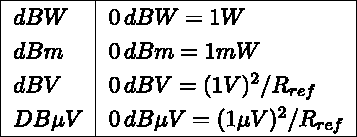
\includegraphics{content/03_Signale/Tabelle2_2.pdf}
	\end{center}
		Bei Spannungspegeln muss Referenzwiderstand berücksichtigt werden. HF üblicherweise 50 $\Omega$, Telefonie 600 $\Omega$
\end{minipage}

\subsubsection{Relative Pegel}
\begin{tabular}{lllr}
	\colorbox{green!30}{\textbf{Spannungspegel}}&  
	$L_u = 20 \cdot \log_{10} \left(\frac{u_x}{u_0}\right)$&
	$U_x = U_0 \cdot 10^{\frac{L}{20}} $ &
	$[L_u] = dB$\\
	
	\textbf{Strompegel}& $L_i  = 20 \cdot \log_{10} \left(\frac{i_x}{i_0}\right)$& $I_x = I_0 \cdot
	10^{\frac{L}{20}} $ & $[L_i] = dB$\\
	
	\colorbox{cyan!30}{\textbf{Leistungspegel}} & $L_P = 10 \cdot \log_{10} \left(\frac{P_x}{P_0}\right)$ & $P_x = P_0 \cdot
	10^{\frac{L}{10}} $ & $[L_P] = dB$ \\
\end{tabular}\renewcommand{\arraystretch}{1}%
\subsubsection{Absolute Pegel}
\begin{tabbing}
	xxxxxxxxxxxxx \= xxxxxxxxxxxxxxxxxxxxxxxxxxxxxxxxxxxxx  \= xxxxxxxxxxxxxxxxxxxxxxx \=\kill
	\colorbox{cyan!30}{\textbf{dBW}} \> Leistungspegel mit Bezugsgrösse $P_0 = $1W \> $\Longrightarrow \: 0 \: dBW = 1W = P_{0_{dBW}}$\\
	\colorbox{cyan!30}{\textbf{dBm}} \> Leistungspegel mit Bezugsgrösse $P_0 = $1mW \> $\Longrightarrow \: 0 \: dBm = 1mW = P_{0_{dBm}}$\\
	\colorbox{green!30}{\textbf{dBV}} \> Spannungspegel mit Bezugsgrösse $U_0 = $1V \> $\Longrightarrow \: 0 \: dBV = P_{0_{dBV}}$\\
	\colorbox{green!30}{\textbf{dB}$\mu$V} \> Spannungspegel mit Bezugsgrösse $U_0 = $1$\mu$V \> $\Longrightarrow \: 0 \: dB \mu V = P_{0_{dB\mu V}}$
\end{tabbing}